\chapter{Analyse}
\section{Contexte}
S'appuyant sur les bases posées dans l'introduction, cette section approfondit l'analyse en commençant par le contexte biologique des espèces de Fusarium.
\subsection{Contexte biologique du genre \textit{Fusarium}}
Depuis un certain temps, les biologistes portent un vif intérêt aux champignons filamenteux du genre \textit{Fusarium}. En effet, les \textit{Fusarium} sont des phytopathogènes qui contaminent, entre autres, les céréales que consomme l’homme comme le blé. Chez ce dernier, ils entraînent la fusariose de l'épi qui détruit les cultures et entraîne des pertes économiques conséquentes. Ces mycètes, sont aussi à l’origine de la contamination des grains par des mycotoxines constituant un problème majeur de sécurité alimentaire. Ces toxines comme les B-trichothécènes sont très stables et se retrouvent dans les grains qui finiront dans l’alimentation.\\

\begin{SCfigure}[1][h]
    \centering
    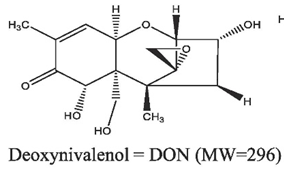
\includegraphics[width=0.25\textwidth]{img/fig_1.png}
    \caption{Formule semi développée du Deoxynivalenol, molécule de la famille des B-trichothécènes produite par les \textit{Fusarium}\cite{gaballah2023development}.}
    \label{fig:mol}
\end{SCfigure}

Jusqu’à présent, le processus de production des mycotoxines a été étudié en ne considérant "qu’un pathogène - une maladie". Cependant, des preuves irréfutables des interactions entre les espèces de \textit{Fusarium} responsables de la fusariose, laisse suggérer que la communication entre ces champignons puisse moduler la régulation de production des toxines.

Afin de mettre en exergue les mécanismes de production de ces molécules inter-individus, il est nécessaire changer d'échelle d'analyse afin d’observer plus globalement le "Meta-Fusarium sp." qui comprend les principales espèces impliquées dans l’infection \cite{ponts2009fusarium, mycsa}. \\

\begin{SCfigure}[1][h]
    \centering
    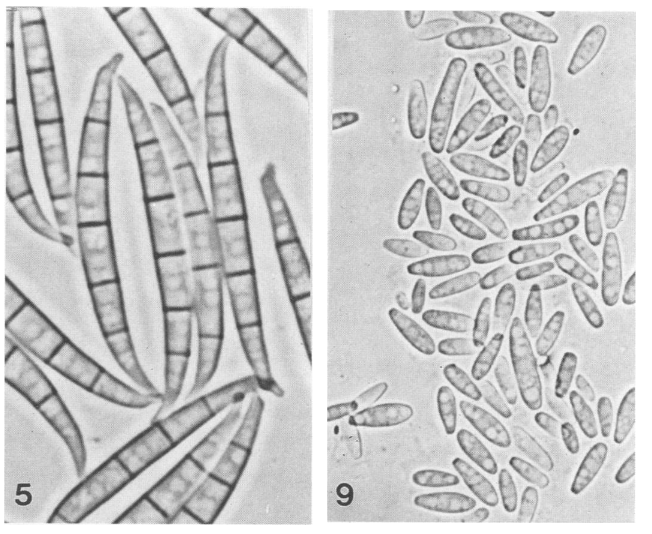
\includegraphics[width=.40\textwidth]{img/fig_2.png}
    \caption{Observation 5 : de macroconidies de \textit{F.graminearum} (950X), 9 : de microcondies de \textit{F.verticillioides} (avant \textit{F.moniliforme} \cite{name}) (1000X) qui sont des champignons qui font partie du Meta-\textit{Fusarium sp} \cite{taxonomy}.}
    \label{fig:fusa}
\end{SCfigure}

\subsection{Communication au sein du Meta-
\textit{Fusarium sp.}}
Au sein du Meta-\textit{Fusarium sp.}. la communication s’effectue en partie par le biais de petits acides ribonucléiques comme les small ARN (smRNA) ou les micro ARN (miRNA). Ces derniers sont des courtes séquences de bases non codantes qui peuvent être séquencées.\\

\begin{figure}[h]
    \centering
    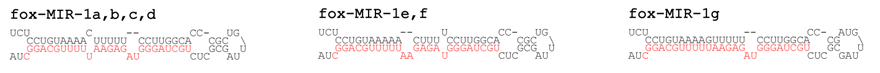
\includegraphics[width=1\textwidth]{img/fig_3.png}
    \caption{Structure secondaire de quelques précurseurs miARN déjà mis en évidence chez les champignons du genre \textit{Fusarium} \cite{chen2014exploring}.}
    \label{fig:mirna}
\end{figure}

Ces petites molécules d'ARN non codantes d'environ 22 nucléotides, sont impliqués dans la régulation post-transcriptionnelle de l'expression génique. En identifiant les miARN spécifiquement produits lors de la communication induite par la rencontre entre deux Fusaria de la même souche, nous pourrons mieux comprendre les mécanismes sous-jacents aux interactions entre les espèces de \textit{Fusarium} toxinogènes. Et ainsi, développer des stratégies de prévention contre la contamination des cultures par les champignons \textit{Fusarium} \cite{ponts2009fusarium, mycsa}.  L’objectif du projet est d’analyser les données séquencées et d’identifier les microARN produits dans chaque scénario de culture, d’en repérer les spécificités et de les quantifier.

\section{État de l'art}
Les pipelines de bio-informatiques visant à gérer des données des séquençages sont très divers et variés. Afin répondre au mieux aux problématiques du client, nous avons réalisé une recherche bibliographique pour rassembler un bouquet d'outils modernes et parfaitement adapté à la tâche. 

L'analyse de données de séquençage de petits ARN dans le contexte de cocultures de céréales et de champignons du genre \textit{Fusarium} nécessite une série d'étapes méthodologiques bien définies. Tout d'abord, l'évaluation de la qualité des données (QC) est essentielle, réalisée grâce à des outils comme FastQC pour obtenir des statistiques détaillées sur la qualité des lectures et MultiQC pour agréger les résultats de plusieurs analyses. Ensuite, le nettoyage des lectures est effectué à l'aide d'outils comme Cutadapt, spécialisé dans l'élimination des adaptateurs, pour préparer les lectures pour l'alignement sur le génome.

L'alignement des lectures sur le génome est une étape cruciale, nécessitant un outil optimisé pour la précision et la gestion des lectures multimappées. BWA-MEM2 est recommandé pour ces raisons. Une fois les lectures alignées, l'identification des petits ARN produits se fait en utilisant ShortStack qui peut annoter ceux déjà connus les ARN connus et isoler les nouveaux, permettant une analyse exhaustive des données. De plus, une indexation des ARN aura lieu grâce à la suite Samtool permettant de gérer les données génomiques de façon très efficace. 

Ces algorithmes se basent sur la recherche de motifs dans des textes grâce à la transformée de Burrows-Wheeler. Elle est à ce jour la méthode algorithmique la plus efficace pour aligner des chaînes de caractères entre elles. 

Le pipeline sera livré sous forme de scripts Python appelant une série de scripts jonglant avec les données.

\section{Présentation des données}

\begin{figure}[ht]
    \centering
    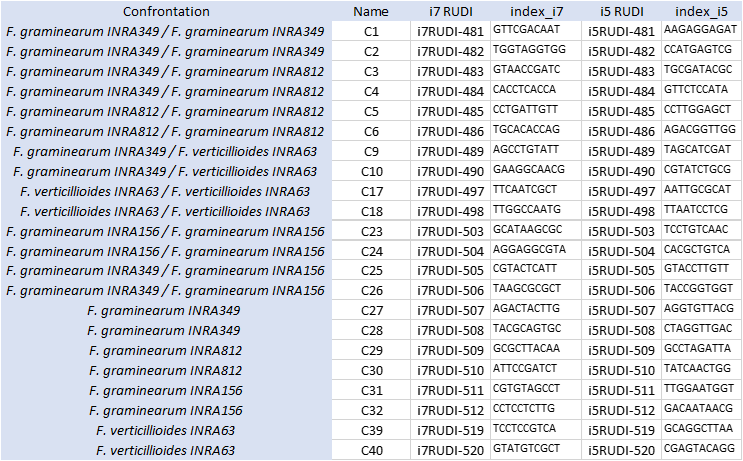
\includegraphics[width=0.8\textwidth]{img/dataset.png}
    \caption{Présentation du jeu de données fourni par le client}
    \label{fig:dataset}
\end{figure}

Pour réaliser ce projet, nous avons travaillé avec un ensemble de données composé de 14 lots en co-culture et 8 lots en mono-culture, comme le montre la figure \ref{fig:dataset}. Ces lots sont des données issues du séquençage Illumina à lecture courte (Short Read), fournies au format FASTQ compressé et désigné par l'extension de fichier ".fastq.gz". Les co-cultures représentent des confrontations entre différentes souches de Fusarium. Les espèces spécifiques utilisées dans cette étude sont Fusarium graminearum, qui comprend les souches INRA349, INRA812 et INRA156, ainsi que Fusarium verticillioides avec la souche INRA63.\\

Chaque lot est identifiée par un nom unique et est associée à des séquences spécifiques, nommées i7 et i5. Ces séquences sont utilisées pour le multiplexage, une technique qui permet d’identifier chaque échantillon de manière unique. Par exemple, la confrontation entre deux souches de F. graminearum INRA349, désignée sous le nom de C1, est associée aux séquences i7 RUDI-481 et i5 RUDI-481.Équipés de données détaillées, nous procédons à l'articulation des besoins spécifiques et des exigences de notre analyse, préparant le terrain pour la conception subséquente de notre pipeline bioinformatique\\


\section{Analyse des besoins}

\subsection{Besoins fonctionnels}
Pour le prétraitement des données, les besoins comprennent :
\begin{itemize}
    \item Acquisition des données issues du séquençage Illumina (Short Read) générées à partir de différentes conditions de culture de Fusarium au format FASTQ.
    \item Prétraitement et nettoyage des données brutes afin d'éliminer les séquences de faible qualité et les erreurs techniques en réalisant un contrôle qualité des lectures.
    \item Normalisation des données.
\end{itemize}

Pour l'analyse des données, les besoins incluent :  
\begin{itemize}
 \item Alignement des lectures prétraitées sur les génomes de référence des souches de Fusarium.
    \item Identifier les miARNs, déterminer leur origine ou leur localisation génomique, et évaluer leur quantité.
    \item Analyse comparative des profils d'expression des microARN entre les échantillons de cultures pures et ceux des confrontations entre souches.
    \item Visualisation des résultats à travers des tableaux et des graphiques codifiés présentant les profils d'expression des miARNs dans les différentes conditions de culture.
\end{itemize}

\subsection{Besoins non fonctionnels}
\begin{itemize}
    \item Utilisation recommandée des langages de programmation adaptés à la bioinformatique, tels que Python, R et éventuellement Bash.
    \item Traitement efficace des données dans des délais raisonnables.
    \item Fiabilité et robustesse pour minimiser les risques de perte de données ou d'erreurs dans l'analyse.
    \item Intuitivité pour une utilisation aisée par les chercheurs non spécialisés en bioinformatique.
    \item Documentation claire et interfaces rationnelles pour faciliter la navigation et l'utilisation des fonctionnalités.
\end{itemize}

\subsection{Contraintes}
\begin{itemize}
    \item Utiliser des outils open source afin d'assurer la transparence, la réutilisabilité du système.
    \item Effectuer nos tâches dans un cadre à accès pseudo-restreint.
    \item Sortir un fichier BigWig compatible avec les plates-formes de navigateur de génome fonctionnelles existantes comme JBrowse pour garantir une visualisation adéquate.
\end{itemize}

\subsection{Ajouts optionnels}
\begin{itemize}
    \item Création d'une base de données pour stocker les résultats.
    \item Sauvegarde et reprise du processus d'analyse et reprise de l'analyse là où elle s'est arrêtée.
    \item Identification des cibles potentielles des miARNs dans les génomes des souches.
\end{itemize}